% ----------------------------------------------------------------------------
% Author: Rayla Kurosaki
% GitHub: https://github.com/rkp1503
% ----------------------------------------------------------------------------

\section{Numerical Simulations}\label{sec:numerical_simulations}
In \myref[Section]{sec:equilibria-analysis}, we used mathematical analysis to compute the equilibria that exists in \myref[Model]{model:rayla-ephraim} and determined the conditions for stability of each one. In this section, we will support and verify the stable equilibria determined in \myref[Section]{sec:equilibria-analysis} through numerical simulations. We will also show the existence of a hopf bifurcation for the interior equilibrium through numerical simulations.

\begin{figure}[H]
    \centering
    \subfloat[$z$-axial equilibrium with the set of parameters~\eqref{params:axial-z}]{%
    \resizebox*{7cm}{!}{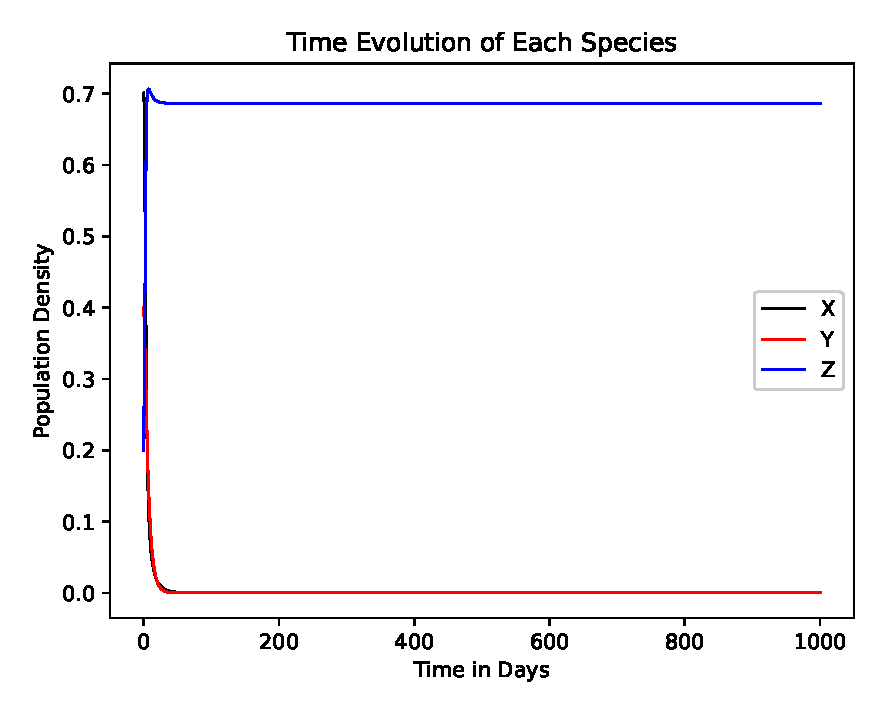
\includegraphics{equilibrium-axial-z}\label{fig:axial-z}}}\hspace{5pt}
    \subfloat[$xy$-boundary equilibrium with the set of parameters~\eqref{params:boundary-xy}]{%
    \resizebox*{7cm}{!}{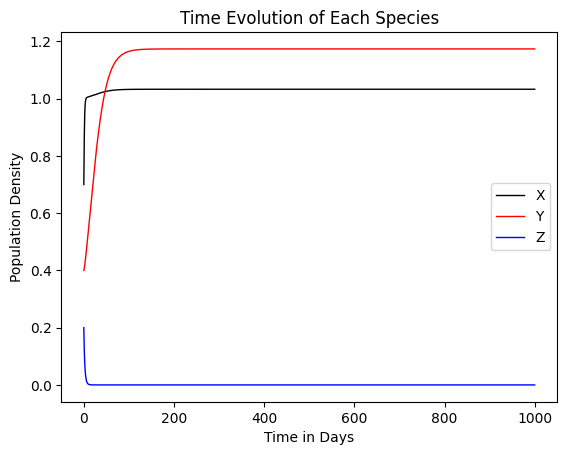
\includegraphics{equilibrium-boundary-xy}\label{fig:boundary-xy}}}\hspace{5pt}
    \subfloat[$xz$-boundary equilibrium with the set of parameters~\eqref{params:boundary-xz}]{%
    \resizebox*{7cm}{!}{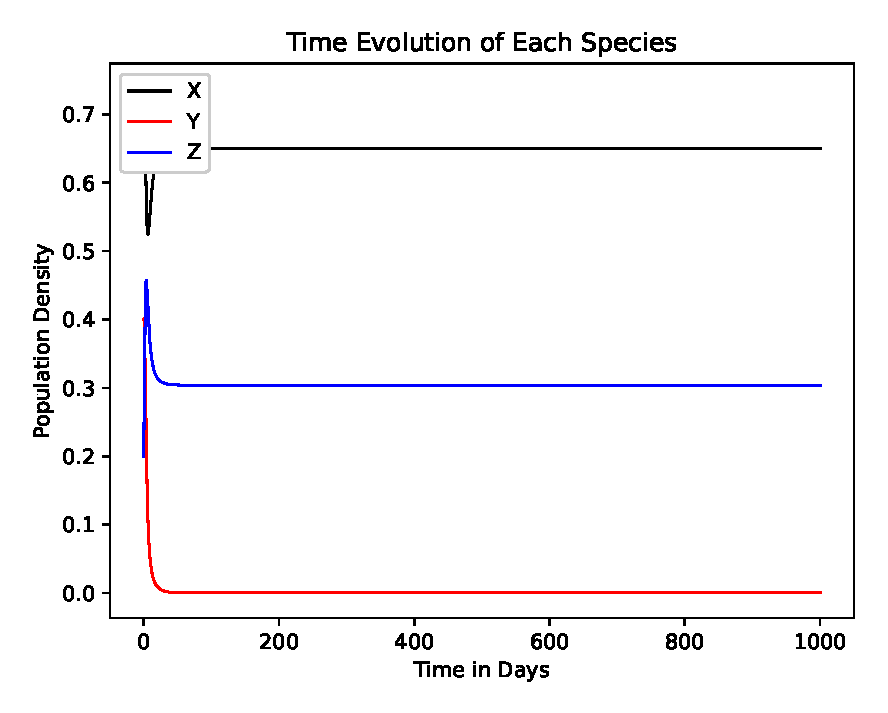
\includegraphics{equilibrium-boundary-xz}\label{fig:boundary-xz}}}\hspace{5pt}
    \subfloat[$yz$-boundary equilibrium with the set of parameters~\eqref{params:boundary-yz}]{%
    \resizebox*{7cm}{!}{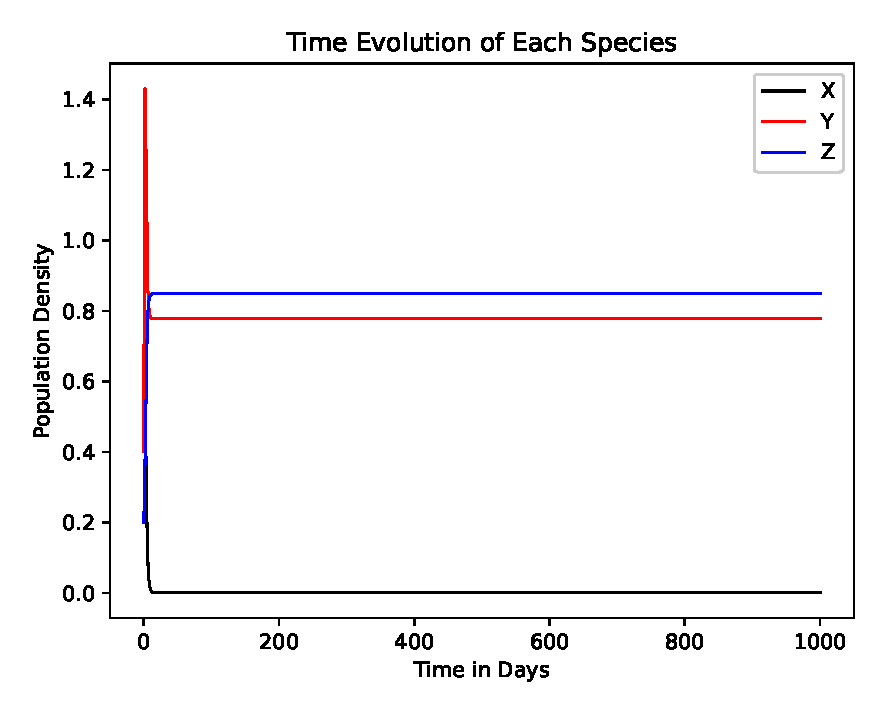
\includegraphics{equilibrium-boundary-yz}\label{fig:boundary-yz}}}
    \caption{Showing the stability of non-interior equilibria for different set of parameters.}
    \label{fig:semi-trivial-equilibria-plots}
\end{figure}

\subsection{The $z$-axial equilibrium}\label{subsec:numsim_z_axial_equilibrium}
By \myref[Theorem]{thm:axial-z-exist} and \myref[Theorem]{thm:axial-z-stability}, we know that the $z$-axial equilibrium
\begin{equation*}
    E_z=\left(0,0,\frac{r_2-v_2}{\gamma_{31}r_2}\right)
\end{equation*}
exists if the condition $r_{zx} > u_4$ is satisfied and is stable if the following conditions are satisfied:
\begin{equation*}
    \frac{u_4}{r_{zx}} < 1-\frac{1}{\varphi_{xz}},\quad
    \frac{u_4}{r_{zx}} < 1-\frac{r_{yx}u_2}{u_1\left(1-p\right)},\quad
    \frac{u_4}{r_{zx}} < \frac{1}{2}
\end{equation*}
To satisfy the conditions above, lets consider the following set of parameters:
\begin{equation}\label{params:axial-z}
    \begin{dcases}
        \begin{aligned}
            r_{yx} &= 0.007\\
            r_{zx} &= 1.136\\
            p &= 0.874
        \end{aligned}
    \end{dcases},\quad 
    \begin{dcases}
        \begin{aligned}
            \varphi_{xy} &= 0.318\\
            \varphi_{yx} &= 0.416\\
            \varphi_{xz} &= 1.59
        \end{aligned}
    \end{dcases},\quad 
    \begin{dcases}
        \begin{aligned}
            u_1 &= 1.655\\
            u_2 &= 0.791\\
            u_3 &= 0.994\\
            u_4 &= 0.356
        \end{aligned}
    \end{dcases}
\end{equation}
Under this set of parameter values, the $z$-axial equilibrium is $E_z=(0,0,0.6866)$. This is further supported by \myref[Figure]{fig:axial-z}, which is the result of numerically solving \myref[Model]{model:rayla-ephraim}.

\subsection{The $xy$-boundary equilibrium}\label{subsec:numsim_xy_boundary_equilibrium}
By \myref[Theorem]{thm:boundary-xy-exist} we know that the $xy$-boundary equilibrium $E_{xy}=\left(x^*,y^*,0\right)$ exists and \myref[Theorem]{thm:boundary-xy-stability} guarantees its stability under appropriate conditions. To satisfy the conditions in \myref[Theorem]{thm:boundary-xy-exist} and \myref[Theorem]{thm:boundary-xy-stability}, we will let $\beta=11$ and consider the following set of parameters:
\begin{equation}\label{params:boundary-xy}
    \begin{dcases}
        \begin{aligned}
            r_{yx} &= 0.049\\
            r_{zx} &= 0.467\\
            p &= 0.645
        \end{aligned}
    \end{dcases},\quad 
    \begin{dcases}
        \begin{aligned}
            \varphi_{xy} &= 0.024\\
            \varphi_{yx} &= 0.163\\
            \varphi_{xz} &= 0.031
        \end{aligned}
    \end{dcases},\quad
    \begin{dcases}
        \begin{aligned}
            u_1 &= 0.31\\
            u_2 &= 0.978\\
            u_3 &= 0.9\\
            u_4 &= 1.004
        \end{aligned}
    \end{dcases}
\end{equation}
Under this set of parameter values, the $xy$-boundary equilibrium is $E_{xy}=(1.0331,1.174,0)$. This is further supported by \myref[Figure]{fig:boundary-xy}, which is the result of numerically solving \myref[Model]{model:rayla-ephraim}.

\subsection{The $xz$-boundary equilibrium}\label{subsec:numsim_xz_boundary_equilibrium}
By \myref[Theorem]{thm:boundary-xz-exist} and \myref[Theorem]{thm:boundary-xz-stability}, we know that the $xz$-boundary equilibrium $E_{xz}=\left(x^*,\ 0,\ z^*\right)$ exist and is locally stable under certain conditions. To satisfy these conditions, lets consider the following set of parameters:
\begin{equation}\label{params:boundary-xz}
    \begin{dcases}
        \begin{aligned}
            r_{yx} &= 0.199\\
            r_{zx} &= 1.494\\
            p &= 0.482
        \end{aligned}
    \end{dcases},\quad 
    \begin{dcases}
        \begin{aligned}
            \varphi_{xy} &= 0.449\\
            \varphi_{yx} &= 0.993\\
            \varphi_{xz} &= 1.152
        \end{aligned}
    \end{dcases},\quad
    \begin{dcases}
        \begin{aligned}
            u_1 &= 1.671\\
            u_2 &= 0.663\\
            u_3 &= 1.556\\
            u_4 &= 1.04
        \end{aligned}
    \end{dcases}
\end{equation}
Under this set of parameter values, the $xz$-boundary equilibrium is $E_{xz}=(0.6499,0,0.3039)$. This is further supported by \myref[Figure]{fig:boundary-xz}, which is the result of numerically solving \myref[Model]{model:rayla-ephraim}.

\subsection{The $yz$-boundary equilibrium}\label{subsec:numsim_yz_boundary_equilibrium}
We also established through \myref[Theorem]{thm:boundary-yz-exist} and \myref[Theorem]{thm:boundary-yz-stability} that the $yz$-boundary equilibrium $E_{yz}=\left(0,\ y^*,\ z^*\right)$ exists and is locally stable respectively, subject to the conditions prescribed in the theorems. To satisfy the conditions in \myref[Theorem]{thm:boundary-yz-exist} and \myref[Theorem]{thm:boundary-yz-stability}, lets consider the following set of parameters:
\begin{equation}\label{params:boundary-yz}
    \begin{dcases}
        \begin{aligned}
            r_{yx} &= 1.219\\
            r_{zx} &= 0.452\\
            p &= 0.589
        \end{aligned}
    \end{dcases},\quad 
    \begin{dcases}
        \begin{aligned}
            \varphi_{xy} &= 0.047\\
            \varphi_{yx} &= 1.587\\
            \varphi_{xz} &= 1.908
        \end{aligned}
    \end{dcases},\quad
    \begin{dcases}
        \begin{aligned}
            u_1 &= 1.658\\
            u_2 &= 1.812\\
            u_3 &= 1.473\\
            u_4 &= 0.289
        \end{aligned}
    \end{dcases}
\end{equation}
Under this set of parameter values, the $yz$-boundary equilibrium is $E_{yz}=(0,0.7773,0.8491)$. This is further supported by \myref[Figure]{fig:boundary-yz}, which is the result of numerically solving \myref[Model]{model:rayla-ephraim}.

\subsection{The interior equilibrium}\label{subsec:numsim_interior_equilibrium}
Finally, in \myref[Theorem]{thm:boundary-yz-exist} and \myref[Theorem]{thm:boundary-yz-stability}, respectively, the existence and stability
of the interior equilibrium $E_{xyz}=\left(x^*,\ y^*,\ z^*\right)$ were established under various sets of conditions. To ensure that the interior equilibrium exist and is stable, lets consider the following set of parameters:
\begin{equation}\label{params:interior-a}
    \begin{dcases}
        \begin{aligned}
            r_{yx} &= 0.5\\
            r_{zx} &= 0.5\\
            p &= 0.6
        \end{aligned}
    \end{dcases},\quad 
    \begin{dcases}
        \begin{aligned}
            \varphi_{xy} &= 0.6\\
            \varphi_{yx} &= 0.15\\
            \varphi_{xz} &= 0.4
        \end{aligned}
    \end{dcases},\quad
    \begin{dcases}
        \begin{aligned}
            u_1 &= 0.6\\
            u_2 &= 0.08\\
            u_3 &= 0.5\\
            u_4 &= 0.5
        \end{aligned}
    \end{dcases}
\end{equation}
Under this set of parameter values, the interior equilibrium is $E_{xyz}=(0.9099,0.0599,0.2305)$. This is further supported by the four figures in \myref[Figure]{fig:nontrivial-equilibria-plots} where \myref[Figure]{fig:time-evolution} shows the time evolution of each Species, \myref[Figure]{fig:phase-plane-3d} shows the phase portrait, and \myref[Figure]{fig:phase-plane-xy}, \myref[Figure]{fig:phase-plane-xz}, and \myref[Figure]{fig:phase-plane-yz} are phase planes when numerically solving \myref[Model]{model:rayla-ephraim}.

For \myref[Model]{model:rayla-ephraim}, we can numerically show that a hopf bifurcation exists for each parameter. Starting with $r_{zx}$, we will plot the time evolution of the ecosystem at $r_{zx}=0.35$ to show that the ecosystem expresses an oscillatory behavior as shown in \myref[Figure]{fig:bifurcation-r_zx-xyz}. Then, we will generate a bifurcation diagram for Species $X,\ Y,\ Z$ over a set interval of $r_{zx}$, expressed in \myref[Figure]{fig:bifurcation-r_zx-x}, \myref[Figure]{fig:bifurcation-r_zx-y}, \myref[Figure]{fig:bifurcation-r_zx-z} respectively. For $r_{zx}$, the interval is $r_{zx}\in(0.133,0.6155)$. From the bifurcation diagrams, we can see that the ecosystem undergoes 2 changes. Denoting the stable solutions for Species $X,\ Y,\ Z$ in black, red, and blue respectively and denoting the unstable solutions in green, we can see that the ecosystem starts off in a stable state and then becomes unstable when $r_{zx}\approx 0.29$. From here, this behavior is maintained until $r_{zx}\approx 0.47$ where it transitions back to a stable state. Thus, we can say that for the set of \myref[parameters]{params:interior-a}, the ecosystem maintains a stable equilibrium when $r_{zx}\in(0.29,0.47)$ and displays an oscillatory behavior when $r_{zx}\in(0.133,0.29)$ and $r_{zx}\in(0.47,0.6155)$.

We can repeat this process using the same set of parameters to show that a hopf bifurcation exists for $p$, $\varphi_{yx}$, and $u_2$. For $p$, the ecosystem undergoes a hopf bifurcation at $p\approx 0.371$, shown in \myref[Figure]{fig:bifurcation-p}. For $\varphi_{yx}$, the ecosystem undergoes a hopf bifurcation at $p\approx 0.387$, shown in \myref[Figure]{fig:bifurcation-phi_yx}. For $u_2$, the ecosystem undergoes a hopf bifurcation at $u_2\approx 0.051$, shown in \myref[Figure]{fig:bifurcation-u_2}. For the other parameters $r_{yx},\ \varphi_{xy},\ \varphi_{xz},\ u_1,\ u_3,\ u_4$, we will consider the set of \myref[parameters]{params:interior-b}. Applying the above procedure to these parameters, we can conclude that the ecosystem undergoes a hopf bifurcation at $r_{yx}\approx 0.66,\ \varphi_{xy}\approx 0.125,\ \varphi_{xz}\approx\{0.402,1.342\},\ u_1\approx 0.728,\ u_3\approx\{0.511,2.501\},\ u_4\approx\{0.122,0.314\}$, depicted in \myref[Figure]{fig:bifurcation-r_yx}, \myref[Figure]{fig:bifurcation-phi_xz}, \myref[Figure]{fig:bifurcation-u_1}, \myref[Figure]{fig:bifurcation-u_3}, \myref[Figure]{fig:bifurcation-u_4} respectively.
\begin{equation}\label{params:interior-b}
    \begin{dcases}
        \begin{aligned}
            r_{yx} &= 0.5\\
            r_{zx} &= 0.5\\
            p &= 0.6
        \end{aligned}
    \end{dcases},\quad 
    \begin{dcases}
        \begin{aligned}
            \varphi_{xy} &= 0.6\\
            \varphi_{yx} &= 0.15\\
            \varphi_{xz} &= 0.4
        \end{aligned}
    \end{dcases},\quad
    \begin{dcases}
        \begin{aligned}
            u_1 &= 0.6\\
            u_2 &= 0.08\\
            u_3 &= 0.5\\
            u_4 &= 0.5
        \end{aligned}
    \end{dcases}
\end{equation}

Similar to the case of varying $r_{zx}$, it can be clearly seen that the simulations given in \myref[Figure]{fig:bifurcation-phi_xz}, \myref[Figure]{fig:bifurcation-u_3} and \myref[Figure]{fig:bifurcation-u_4} show the interior equilibrium undergoing two Hopf bifurcations for each of the parameters indicated. In particular, we observe that increasing values of $r_{zx}$ and $u_3$ beyond the ranges provided will lead to the collapse of species $Y$. These are other bifurcations where the interior equilibrium changes into the xz-boundary equilibrium.  The model’s prediction of the eventual collapse of the $Y$ species given a further increase in the values of $r_{zx}$ and $u_3$ is as expected since these are the parameters associated with, respectively,  the growth rate and attack rate of species $Z$ that is preying on $Y$. We also observed that further increase in the value of the amensalism parameter $varphi_{xz}$ will lead to the demise of species $X$ and  as a consequence, the interior equilibrium will collapse into yz-boundary equilibrium. Another bifurcation we observed is that a further increase in the value of the parameter $u_4$ that is related to the decay rate of species $Z$ will lead to its eradication and the interior equilibrium will become the xy-boundary equilibrium. 
